\chapter{SRS DOCUMENT} \label{ch:procedure}
\section{Chapter 1}

\subsection*{Introduction}

The rapid growth of digital commerce has transformed the way small businesses operate, with many entrepreneurs relying heavily on social media platforms such as Facebook and WhatsApp to reach customers. While these platforms are effective for marketing and communication, they lack essential features for structured order management, inventory control, and business analytics. As a result, small vendors often struggle to scale their operations efficiently.

The Multi-Tenant E-Commerce System is proposed as a Software as a Service (SaaS) platform designed to bridge this gap. The system enables multiple vendors to register and instantly obtain their own personalized online storefront without the need for technical expertise. By employing a multi-tenant architecture, the platform ensures efficient resource usage while keeping each vendor’s data isolated and secure. This solution empowers small business owners to manage their products, customers, and orders professionally, while significantly reducing the cost and complexity of building and maintaining individual e-commerce websites.

\subsection{Purpose}
The purpose of this Software Requirements Specification (SRS) is to define the functional and non-functional requirements for the Multi-Tenant E-Commerce System. This document outlines the architectural constraints and behavioral specifications necessary to build a "Software as a Service" (SaaS) platform that empowers small vendors, specifically Social Commerce entrepreneurs (operating on platforms like Facebook and Instagram), to launch dedicated online storefronts without technical expertise.

The primary objective of the system described in this document is to automate the manual order-taking process currently used by small vendors. By leveraging a multi-tenant architecture, the system allows a "Super Admin" to host a single application instance that serves multiple "Tenants" (Vendors), providing each with a unique URL, rigorous data isolation, and a personalized storefront experience.

This document serves as the authoritative source for the system's requirements and validation criteria. It is intended for:
\begin{itemize}
    \item \textbf{Developers:} To understand the functional specifications, data isolation requirements, and user interface constraints necessary for development.
    \item \textbf{Project Supervisors \& Reviewers:} To verify that the proposed system meets academic standards and fulfills the objectives outlined in the project proposal.
    \item \textbf{Quality Assurance:} To define the testing criteria and expected system behaviors for user acceptance testing.
\end{itemize}

\subsection{Intended Audience}

The primary intended audience of the Multi-Tenant E-Commerce System is small business owners, new entrepreneurs, and F-commerce sellers who primarily operate through platforms like Facebook and WhatsApp. These individuals often lack the financial resources and technical knowledge required to develop and maintain a full-scale e-commerce website. This system is designed to support vendors who want to professionalize their business, manage orders and products more efficiently, and build a stronger online presence without the burden of high development costs. Additionally, the platform can benefit freelancers, home-based businesses, and local sellers who wish to expand digitally with minimal investment. 

\subsection{Intended Use}

The Multi-Tenant E-Commerce System is intended to serve as a cloud-based digital commerce platform that supports small and medium-sized businesses in managing and growing their online operations. The system is designed primarily for sellers who currently rely on social media platforms such as Facebook, Instagram, and WhatsApp for conducting business but lack structured tools for managing customers, orders, and inventory.

The platform will be used by business owners to create and manage their own branded online storefronts, where they can display products, track stock levels, process customer orders, and monitor sales activity. In addition, the system will provide integrated access to verified wholesale suppliers, enabling sellers to restock products directly through the same platform without needing to search for suppliers separately.

Wholesale suppliers will use the system to list products in bulk, manage available inventory, and receive purchase orders from registered sellers. End customers will interact with the platform indirectly through individual seller storefronts, where they can browse products, place orders, and complete purchases.

The system is intended to be accessed through standard web browsers and mobile devices, ensuring usability for individuals with limited technical knowledge and primarily mobile-based internet access. Overall, the intended use of the system is to simplify digital commerce operations, reduce manual workload, and create a more organized and scalable business environment for small online sellers.

\subsection{Product Scope}  
So, the Multi-Tenant E-Commerce System is basically a cloud-based system which is supposed to allow small business owners to get a leg up, especially those who are kinda floundering with social media trying to find and deal with customers and sales. We're trying to give them one digital storefront.It's an instructable pan in which a business owner can post stuff, keep track of inventory, ship orders, all under their own branded online shop.

Benefits:  
\begin{itemize}
For Small Businesspersons (Tenants):  
    \item \textbf{Customer Acquisition \& Retention:} Among others, it transcends the limitations of Instagram, Facebook or TikTok\'s algorithms as it could offer a polished and dedicated online store that increases discover-ability and credibility.  
    \item \textbf{Operational Efficiency:} Sweeps up all questions, orders, payments by customers - Facebook, Insta, WhatsApp - into one tidy dashboard. 
    \item \textbf{Reduced administrative Hassle:} Chess (like tracking inventory, tracking orders, and rudimentary sales reports) occurs automatically.  
    \item \textbf{Low Barrier to Entry:} Provides an affordable, scalable solution to creating a custom e-com platform, and you don't need to be a tech wizard.  
\end{itemize}
\textbf{Objectives \& Goals:}
\begin{enumerate}
    \item \textbf{Primary Objective:} Pump up sales and reduce operational headaches for small, social media heavy businesses by launching an all in one e-commerce platform.  
    \item \textbf{Technical Goal:} Developing a safe, scalable and reliable multi-tenant architecture in which the data of each tenant is completely isolated - but the entire system is maintained and updated from a single codebase.
    \item \textbf{User Experience Goal:} Deliver a snappy, mobile-first interface that doesn't need hours of training. Let's say that your tenant wants to get their store up and running in a few hours.  
\end{enumerate}

\textbf{Overall Business Goals:}  
This SRS document and resultant software play an important role in hitting the organization's strategic business targets:  
\begin{itemize}
    \item \textbf{Market Penetration:} Provides an obvious product to acquire a sizeable chunk of the non-serve segment of digitally-natives in small-business owners.  
    \item \textbf{Brand Establishment:} Positions us as a go-to facilitate small-biz digital transformation in the region.  
    \item \textbf{Cross-Functional Alignment:} This SRS provides context to teams that are outside of development:  
\end{itemize}
\textbf{Marketing \& Sales:} Use the features and benefits to build targeted marketing campaigns, sales collateral and explain the value for both tenants and suppliers. 

\textbf{Customer Support:} Refer to the system's capabilities and user goals in building training materials, help docs, and supporting protocols.  

\textbf{Leadership/management:} How to use the stated objectives and goals to track the success of the project and to steer future investments and decisions about the road map. 

Finally, the scope of this product is to create a simple yet complex platform which reverses the way small social-centric businesses operate, which directly pushes the company's mission of expanding access to digital commerce as well as creating a sustainable SaaS business model.

\subsection{Risk Definition}
A risk is any potential issue that may negatively impact the system’s security, legality, performance, or user trust during development or operation.

\begin{enumerate}
    \item \textbf{Illegal Product Listing Risk} \\
    Vendors may attempt to sell illegal products such as drugs, weapons, or restricted items through the platform. \\
    \textbf{Impact:} Legal issues, platform misuse, and damage to system credibility.

    \item \textbf{Fake or Invalid Payment Risk} \\
    Customers may attempt to make payments using fake, invalid, or fraudulent money or payment methods. \\
    \textbf{Impact:} Financial loss and disputes between vendors and customers.

    \item \textbf{Payment Dispute Risk} \\
    Conflicts may arise regarding payment confirmation, delayed payments, or incomplete transactions. \\
    \textbf{Impact:} Customer dissatisfaction and trust issues with the platform.

    \item \textbf{Product Return and Refund Dispute Risk} \\
    Disagreements may occur between vendors and customers regarding product returns, refunds, or damaged goods. \\
    \textbf{Impact:} Increased complaints and operational complexity.

    \item \textbf{Data Security and Privacy Risk} \\
    There is a risk of unauthorized access to vendor or customer data if proper security controls are not implemented. \\
    \textbf{Impact:} Data breaches and loss of user trust.

    \item \textbf{Vendor Misuse Risk} \\
    Some vendors may misuse the platform by providing false product information or misleading customers. \\
    \textbf{Impact:} Reduced reliability and customer confidence.

    \item \textbf{User Adoption Risk} \\
    Vendors may prefer continuing business through social media instead of adopting a new platform. \\
    \textbf{Impact:} Low platform usage and limited success.

    \item \textbf{Fraudulent Order and Cancellation Risk} \\
    Users may place false or spam orders, such as booking Cash on Delivery (COD) items with no intention of accepting delivery, or repeatedly creating and canceling orders to disrupt operations. \\
    \textbf{Impact:} Financial loss due to wasted shipping costs, inventory mismanagement (locking stock from real buyers), and increased operational overhead.
\end{enumerate}

\section{Chapter 2}
\subsection{User Classes and Characteristics}
\label{sec:user-classes}
The Multi-Tenant E-Commerce System interacts with three distinct user classes. These classes are differentiated by their access levels, technical proficiency, and frequency of interaction with the platform.

\subsection*{Super Admin (System Operator)}
\label{subsec:super-admin}
The Super Admin is the primary stakeholder responsible for the maintenance and business viability of the SaaS platform. This user does not engage in commerce but rather facilitates the ecosystem for Tenants.

\begin{table}[H]
\centering
\begin{tabular}{|p{4.5cm}|p{10cm}|}
\hline
\textbf{Characteristic} & \textbf{Description} \\
\hline
\textbf{Role} & System Administrator and Business Owner. \\
\hline
\textbf{Responsibilities} & Monitoring server health, managing tenant subscriptions, enforcing platform policies (banning illegal items), and resolving high-level disputes. \\
\hline
\textbf{Technical Proficiency} & High. Expert understanding of web technologies, dashboard analytics, and administrative configurations. \\
\hline
\textbf{Frequency of Use} & Continuous. Daily access is required to monitor system stability and security logs. \\
\hline
\textbf{Education/Background} & Typically IT professionals or business administrators with experience in SaaS management. \\
\hline
\end{tabular}
\caption{Super Admin Characteristics}
\label{tab:super-admin}
\end{table}

\subsection*{Tenant (Vendor)}
\label{subsec:tenant}
The Tenant is the core user of the system—a small business entrepreneur utilizing the platform to professionalize their existing S-commerce (Social Commerce) operations.

\begin{table}[H]
\centering
\begin{tabular}{|p{4.5cm}|p{10cm}|}
\hline
\textbf{Characteristic} & \textbf{Description} \\
\hline
\textbf{Role} & Storefront Manager and Seller. \\
\hline
\textbf{Responsibilities} & Creating the store, uploading products, managing inventory, processing orders, and handling customer inquiries. \\
\hline
\textbf{Technical Proficiency} & Low to Moderate. Highly proficient with mobile apps (Facebook/Instagram/WhatsApp) but lacks formal IT training or experience with complex web CMS platforms. \\
\hline
\textbf{Frequency of Use} & High/Daily. Constantly logged in via mobile devices to track sales and stock levels. \\
\hline
\textbf{Education/Background} & Varied background (home-based business owners, students, local traders). They require a low-code/no-code interface. \\
\hline
\end{tabular}
\caption{Tenant (Vendor) Characteristics}
\label{tab:tenant}
\end{table}

\subsection*{End Customer (Shopper)}
\label{subsec:end-customer}
The End Customer is the external user who purchases goods. They view the Tenant’s storefront as an independent brand and may be unaware of the underlying SaaS provider.

\begin{table}[H]
\centering
\begin{tabular}{|p{4.5cm}|p{10cm}|}
\hline
\textbf{Characteristic} & \textbf{Description} \\
\hline
\textbf{Role} & Buyer / Consumer. \\
\hline
\textbf{Responsibilities} & Browsing catalogs, adding items to cart, providing shipping details, and making payments. \\
\hline
\textbf{Technical Proficiency} & Varied. Ranges from digital natives to novice internet users. The interface must be intuitive enough for users with minimal digital literacy. \\
\hline
\textbf{Frequency of Use} & Variable. Usage is sporadic, driven by marketing campaigns or specific purchasing needs. \\
\hline
\textbf{Education/Background} & General public. \\
\hline
\end{tabular}
\caption{End Customer Characteristics}
\label{tab:end-customer}
\end{table}

\subsection{User Needs}
\label{subsec:user-needs}

The Multi-Tenant E-Commerce System is designed to fulfill the needs of different types of users, including vendors, customers, and system administrators. The system aims to provide an easy-to-use, secure, and efficient platform for managing online business operations.

\subsubsection{Vendor Needs}
\label{subsec:vendor-needs}

Vendors require a platform that allows them to easily create and manage their own online storefront without technical knowledge. Vendors need the ability to add, update, and remove products, manage inventory, track orders, and communicate with customers. They also require secure access to their business data and a simple interface for monitoring sales and order status. Finding and reaching customers easily without extra hassles of different social media platforms is also a necessary requirement.

\subsubsection{Customer Needs}
\label{subsec:customer-needs}

Customers need a convenient and reliable platform to browse products from different vendors, view product details, place orders, and track purchase status. They require secure payment options, clear product information, and a user-friendly interface to ensure a smooth shopping experience.

\subsubsection{Administrator Needs}
\label{subsec:administrator-needs}

System administrators need tools to monitor platform activities, manage vendor registrations, and ensure compliance with system policies. They require the ability to monitor transactions, control system security, and prevent illegal or inappropriate product listings. Administrators also need to maintain system stability and manage user accounts when necessary.

\subsection{Operating Environment}

The Multi-Tenant E-Commerce System will operate as a cloud-based web application hosted on a scalable server infrastructure and delivered through a single system deployment. All vendors will use the same core frontend and backend system, ensuring consistency, maintainability, and efficient updates, while still allowing individual tenants to apply customizable themes, branding, and configuration settings to personalize their storefronts. The platform will be accessible through modern web browsers on desktops and mobile devices without requiring any additional software installation and will support common operating systems such as Windows, Linux, Android, and iOS. A stable internet connection will be required, as all business data, including orders, inventory, and product tracking information, will be processed and stored on the cloud servers. The system will include product tracking functionality that enables vendors and customers to monitor order status and shipment progress through integrated logistics or tracking services. The cloud-based operating environment is designed to support secure communication, third-party integrations such as payment gateways and delivery providers, and scalable operation as the number of tenants and transactions grows.


\subsection{Constraints}

This section describes the predefined design, implementation and operational boundaries that the Multi-Tenant E-Commerce System needs to follow. These constraints are non-negotiable, and comprise the basic framework for the project.
    \subsubsection{Architectural Constraints}

    \textbf{Multi-Tenant SaaS Model:} The system must be coded and deployed as single and shared Software-as-a-Service (SaaS) application for multiple independent vendors (tenants). A monolithic or single tenant architecture is strictly prohibited.

    \textbf{Data Isolation:} The system has to support strict logical data isolation between tenants at the database level. Data from one vendor should be totally inaccessible and invisible to all the other vendors under normal application usage. Physical database separation per tenant is not allowed because of scalability and maintenance overhead.

    \textbf{Shared Application Instance:} All tenants shall be served from the same application codebase and server instance. Separate codebases or instances of servers for individual vendors are not permitted.


    \subsubsection{Design and Implementation Limitations}

    \textbf{Super Admin Need:} A system must have a special "Super Admin" portal to manage the platform, including supervising tenant onboarding, platform-wide configuration, and system health monitoring.

    \textbf{Instant Tenant Onboarding:} After successful registration and subscription, a new vendor must be given instant access into a full featured, personalized admin panel with a live, publicly accessible storefront URL. For standard onboarding flow manual configuration or setup delays for Super Admin are not allowed.

    \textbf{No Custom Code per Tenant:} The system should not support tenant-specific custom code deployment. All the customization for a vendor's storefront (e.g. colors, logo, banner) is required to be done via configuration settings and theme options within the shared application.
    
    \textbf{Order and shipment boundary:} As this platform is only for Bangladeshi tenant so order and delivery is not allowed in abroad. It has to be used within Bangladesh.	

    \textbf{Preset Payment Gateways:} Vendor storefronts are required to integrate with a predefined and limited set of payment gateways (e.g. bKash, Nagad) at the platform level. The system will not support the integration of arbitrary, vendor specific payment processors.

\subsection{Project Assumption}
\label{sec:project-assumption}

Assumptions are conditions that are believed to be true for the successful development and operation of the system.

\begin{enumerate}
    \item \textbf{Internet Availability Assumption:} It is assumed that vendors and customers will have access to a stable internet connection to use the platform.
    
    \item \textbf{Legal Business Usage Assumption:} It is assumed that vendors will use the platform only to sell legal and permitted products and will follow local laws and regulations.
    
    \item \textbf{Vendor Responsibility Assumption:} It is assumed that vendors are responsible for managing their own products, prices, inventory, and order fulfillment.
    
    \item \textbf{Payment System Reliability Assumption:} It is assumed that integrated payment methods will function correctly and provide accurate transaction information.
    
    \item \textbf{User Honesty Assumption:} It is assumed that vendors and customers will provide correct and truthful information during registration and transactions.
    
    \item \textbf{Basic Technical Knowledge Assumption:} It is assumed that vendors have basic knowledge of using smartphones or web applications.
    
    \item \textbf{System Usage Policy Assumption:} It is assumed that users will follow the platform's terms, conditions, and usage policies.
    
    \item \textbf{Single Platform Maintenance Assumption:} It is assumed that the system will be maintained and updated by the platform administrator.
    
    \item \textbf{Browser Compatibility Assumption:} It is assumed that users will access the system using modern web browsers.
\end{enumerate}
%\begin{figure}[H]
%    \centering
%    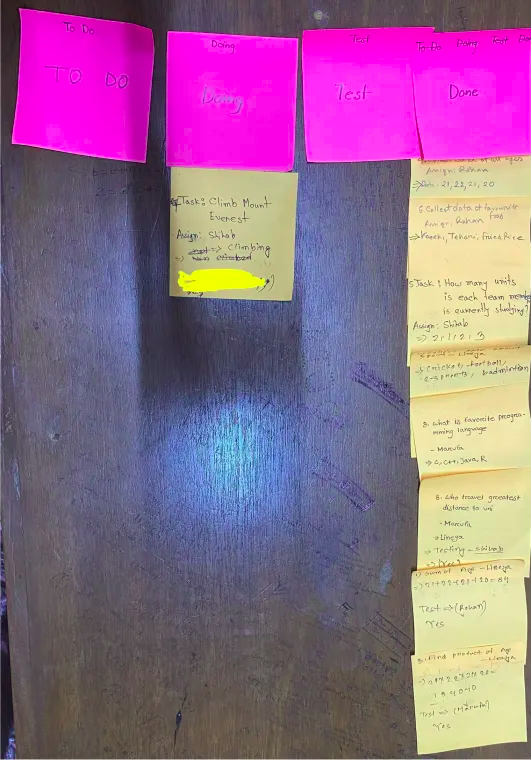
\includegraphics[width=0.5\linewidth]{figures/phase-5.png}
%    \caption{Phase 5}
%    \label{fig:placeholder}
%\end{figure}